\begin{figure*}[t]
	\centering
\begin{subfigure}[t]{0.33\linewidth}
		\centering
		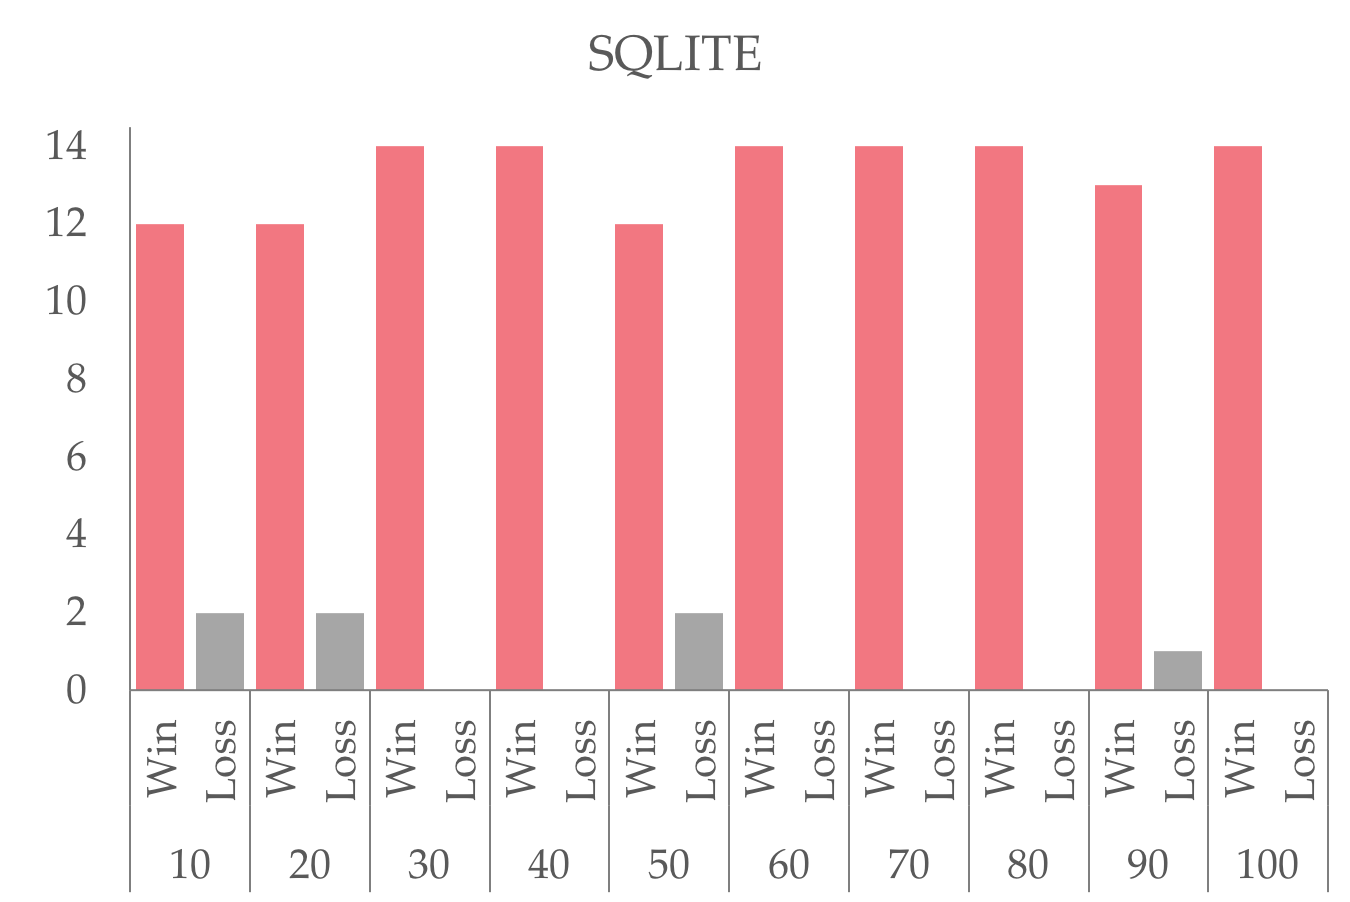
\includegraphics[width=\linewidth]{figures/sqlite_rq2.png}
\end{subfigure}%
\begin{subfigure}[t]{0.33\linewidth}
		\centering
		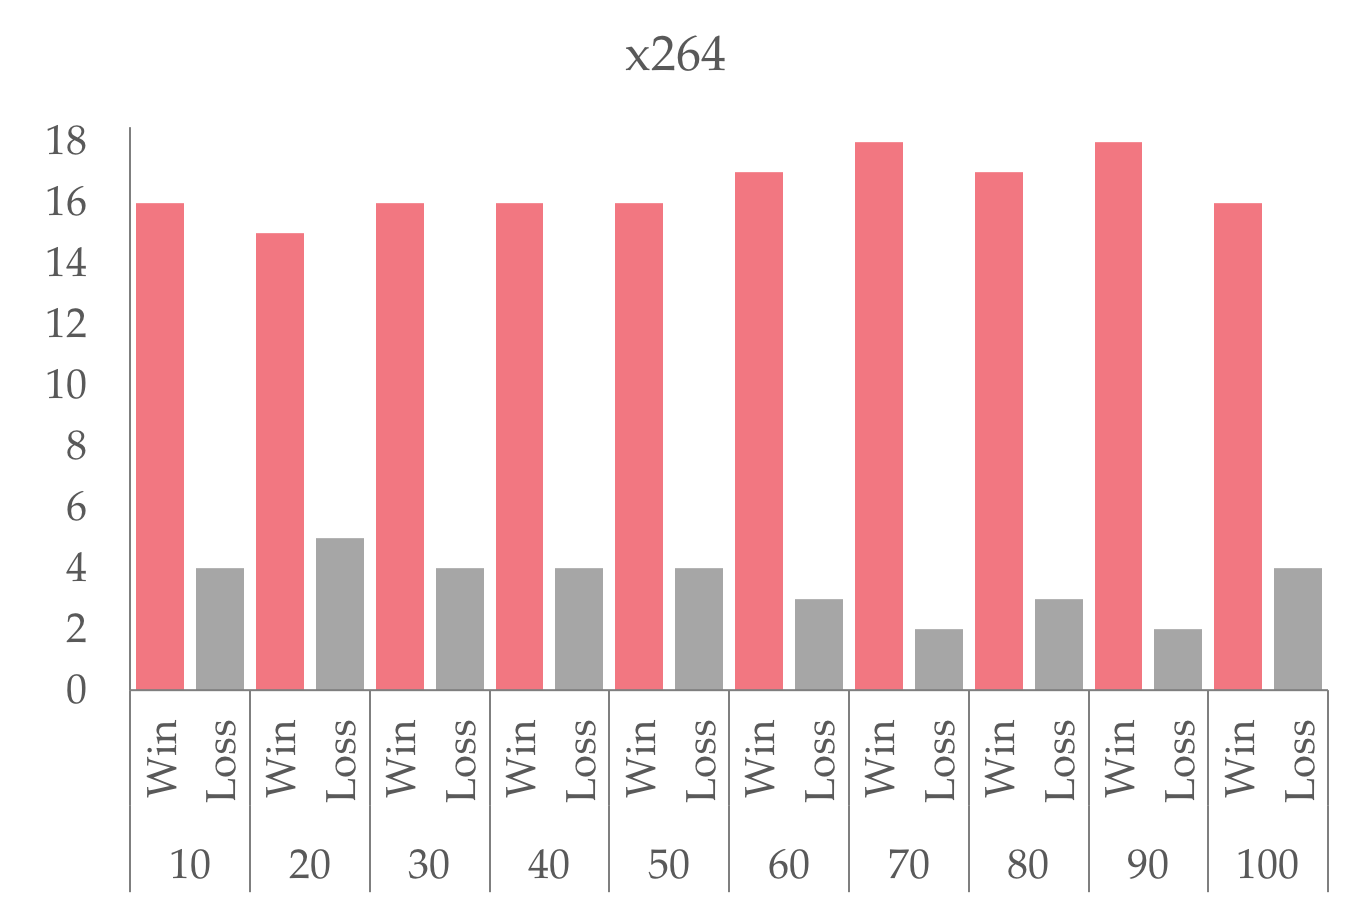
\includegraphics[width=\linewidth]{figures/x264_rq2.png}
\end{subfigure}%
\begin{subfigure}[t]{0.33\linewidth}
		\centering
		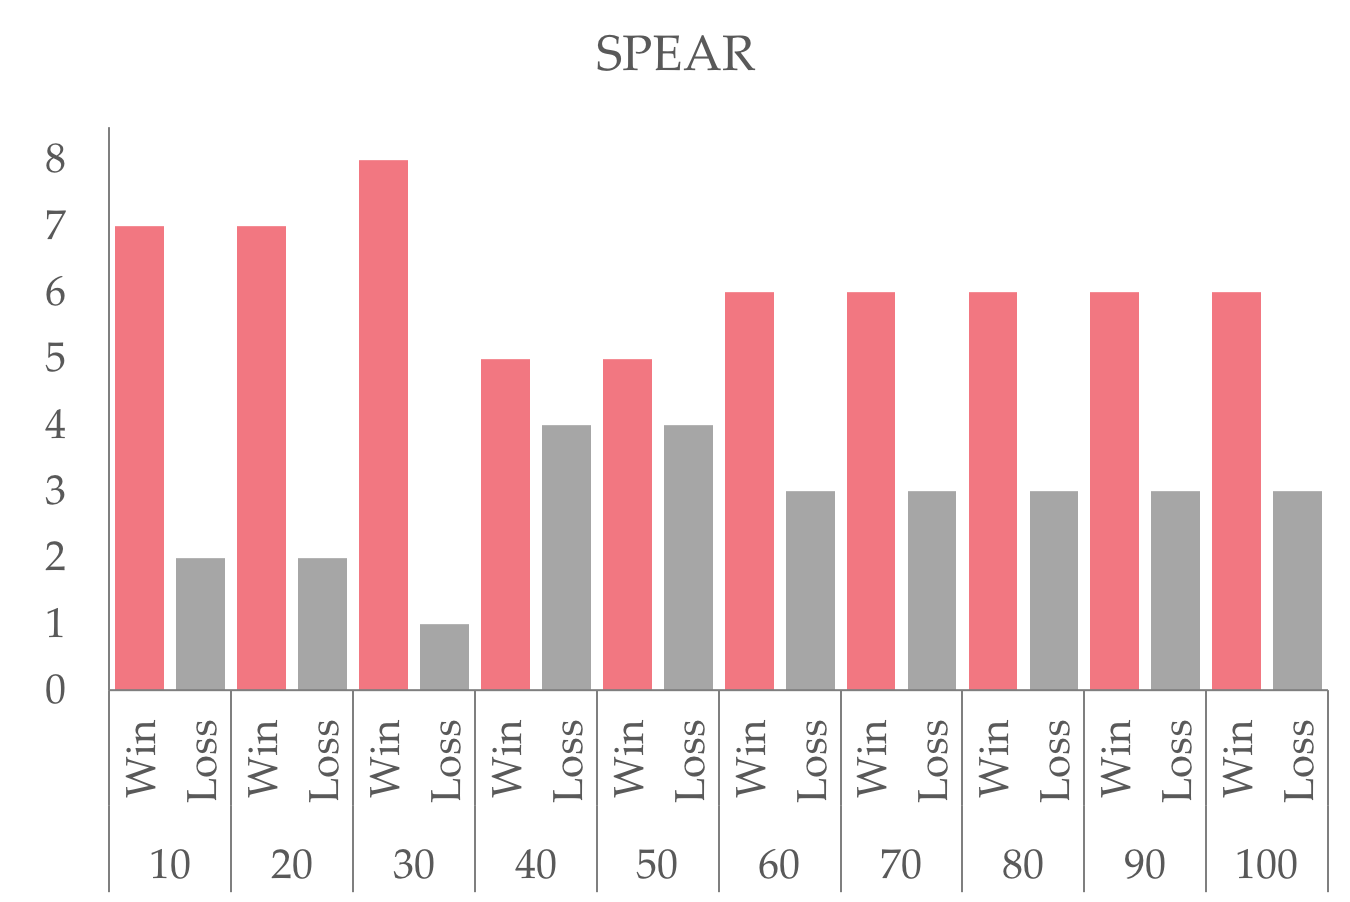
\includegraphics[width=\linewidth]{figures/spear_rq2.png}
\end{subfigure}\\[0.25cm]
\begin{subfigure}[t]{0.33\linewidth}
		\centering
		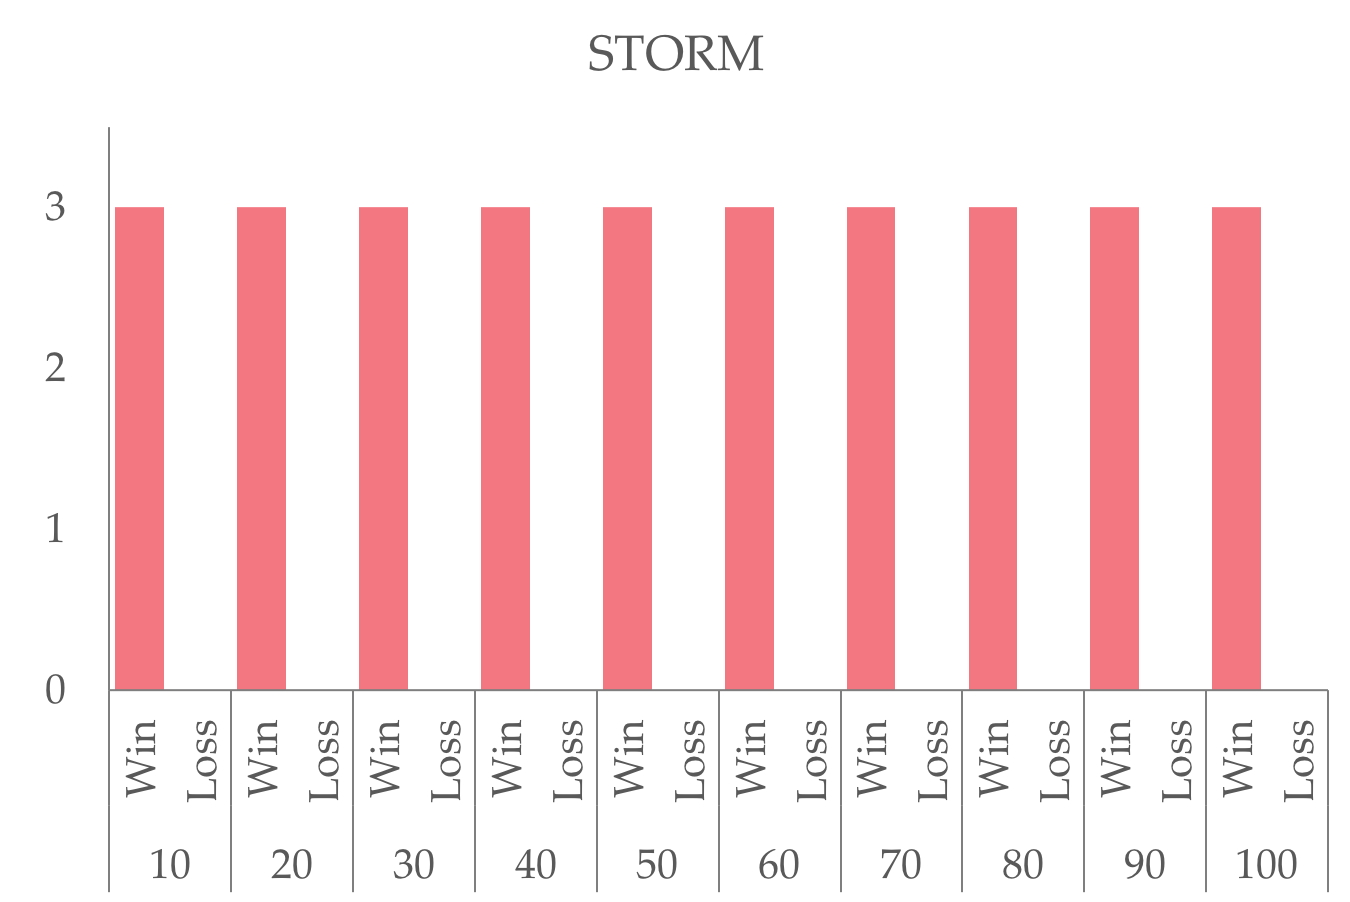
\includegraphics[width=\linewidth]{figures/storm_rq2.png}
\end{subfigure}\hspace{12pt}
\begin{subfigure}[t]{0.33\linewidth}
		\centering
		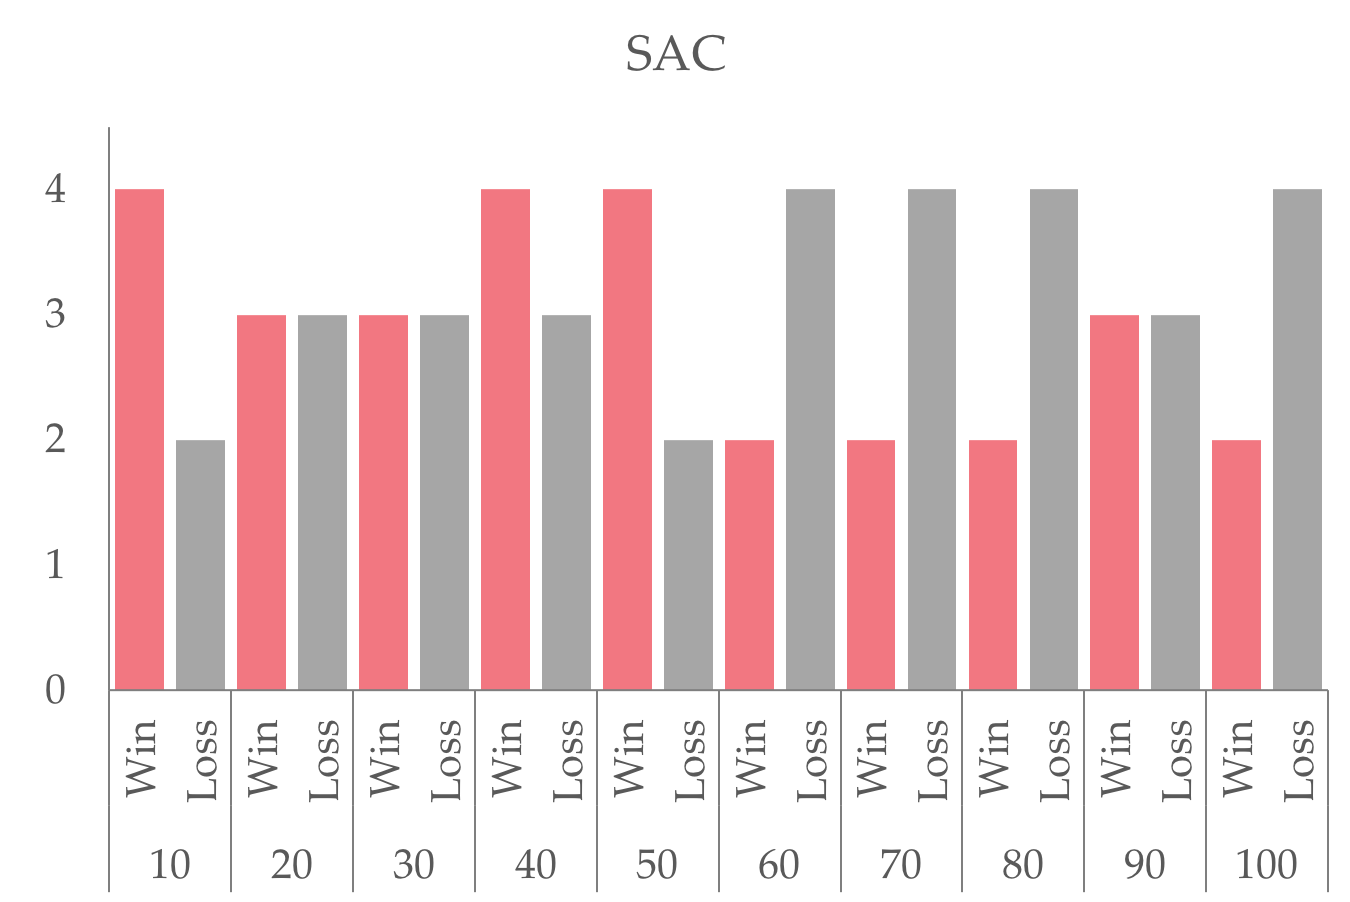
\includegraphics[width=\linewidth]{figures/sac_rq2.png}
\end{subfigure}\\[0.25cm]
	\caption{{\small Win/Loss analysis of learning from the bellwether environment and target environment using Scott Knott. The x-axis represents the percentage of data used to build a model and y-axis is the count.
	BEETLE wins in all models except for SAC-- and there only there when we have measured 50+\% of the data.}}
	\label{fig:rq2_1}
\end{figure*}
